\chapter[Diseño del hardware]{Diseño del hardware\label{cap:hardware}}

El hardware del prototipo se organiza como una estación compacta de
observación solar, con operación local y sincronización remota. La
Raspberry Pi 5 concentra las funciones de control, adquisición,
preprocesamiento y comunicación, mientras que la cámara ZWO ASI174MM Mini y el
prisma Herschel wedge con filtro ND3.0 conforman el bloque óptico para captura
fotosférica en luz blanca.

La arquitectura integra cámara, pantalla local de estado, refrigeración activa,
conectividad inalámbrica y almacenamiento temporal en un nodo embebido único.
Esta disposición permite operar el instrumento aun sin conexión permanente a
Internet y reservar la sincronización con la plataforma web para los periodos en
que el enlace esté disponible. La Figura~\ref{fig:esquema_electrico_general_hardware}
resume la integración eléctrica entre la Raspberry Pi 5 y los elementos
principales del prototipo.

\begin{figure}[H]
    \centering
    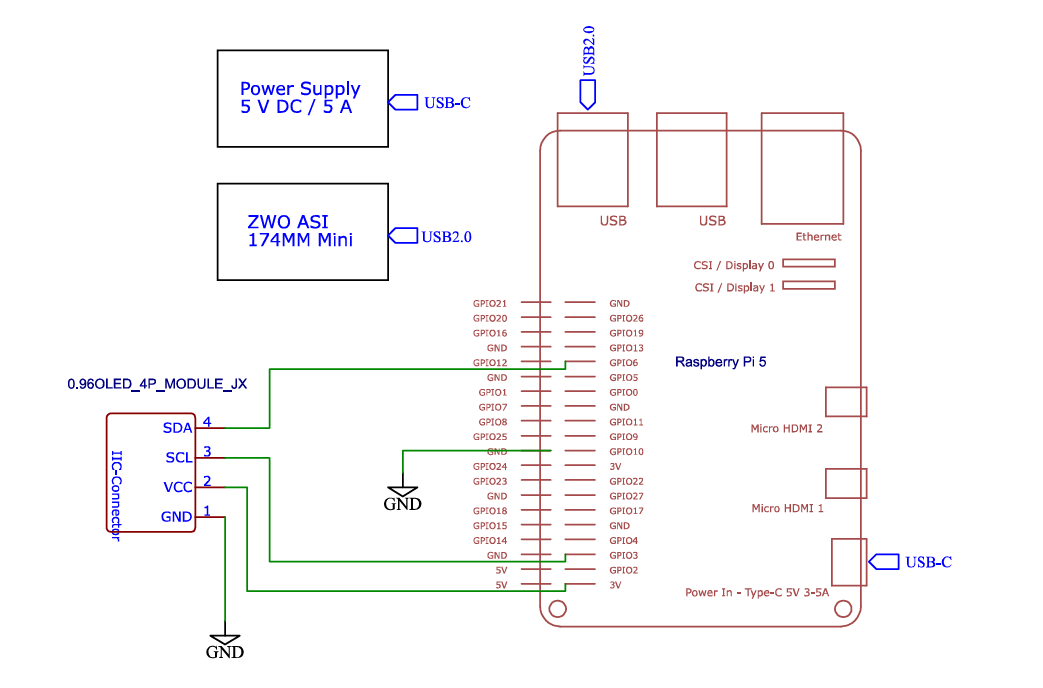
\includegraphics[width=0.90\textwidth]{figures/hw/electric.png}
    \caption{Esquema eléctrico general del sistema de adquisición, mostrando la
    Raspberry Pi 5 como unidad central. \textbf{Fuente:} Elaboración propia.}
    \label{fig:esquema_electrico_general_hardware}
\end{figure}

\section{Unidad de procesamiento embebido}

La implementación adopta una Raspberry Pi 5 de 8\,GB como unidad de
procesamiento embebido, en concordancia con los criterios de selección expuestos
en la Tabla~\ref{tab:comparacion_plataformas_embebidas}. Esta placa cumple el rol
de nodo de borde (\textit{edge computing}): inicializa los servicios de
adquisición, gestiona la cámara, ejecuta el preprocesamiento local y almacena de
forma temporal capturas, metadatos e inferencias preliminares.

La conectividad combina un punto de acceso local mediante \textit{hotspot}, para
configuración y monitoreo en campo, con enlace WiFi hacia una red disponible para
sincronización posterior con la plataforma web y la base de datos en la nube
\cite{raspberryPi5Docs2026,nmcliHotspot2026}. Debido a la ejecución continua de
adquisición, transferencia y preprocesamiento, se incorpora refrigeración activa
(\textit{active cooler}) para mejorar la disipación térmica y reducir eventos de
\textit{thermal throttling} durante sesiones prolongadas.

\begin{figure}[H]
    \centering
    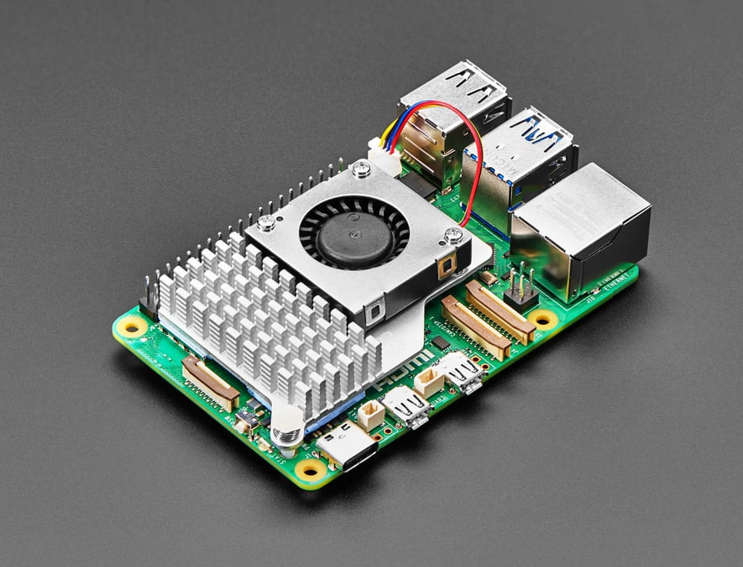
\includegraphics[width=0.70\textwidth]{figures/hw/cooler.png}
    \caption{Raspberry Pi 5 de 8\,GB con sistema de refrigeración activa,
    empleada como unidad de procesamiento embebido para captura,
    preprocesamiento local, inferencia preliminar y sincronización con la nube. \textbf{Fuente:} página oficial de Raspberry Pi.}
    \label{fig:raspberry_pi5_nodo_borde}
\end{figure}

\subsection{Pantalla local de estado}

Como interfaz auxiliar se emplea una pantalla OLED de \(0.96''\) y resolución
\(128\times64\) píxeles. Su función es entregar diagnóstico inmediato en campo:
estado de red, disponibilidad del \textit{hotspot}, detección de cámara,
ejecución del servicio de adquisición y avisos básicos de error. De este modo, el
operador puede verificar el estado del nodo sin recurrir a un monitor externo,
una sesión SSH ni la plataforma web.

La comunicación con la Raspberry Pi 5 se realiza mediante bus I2C, reduciendo la
interconexión a dos líneas de datos/control y dos líneas de alimentación. La
Tabla~\ref{tab:conexionado_oled_pi5} resume el conexionado empleado.

\begin{figure}[H]
    \centering
    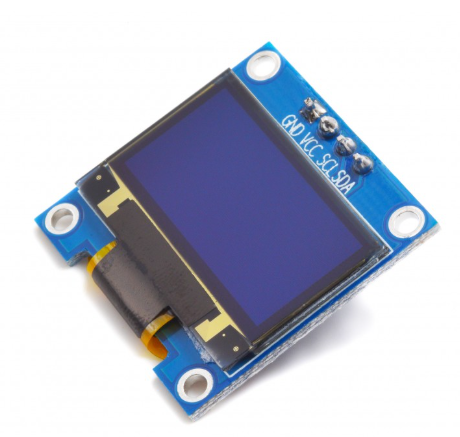
\includegraphics[width=0.55\textwidth]{figures/hw/oled.png}
    \caption{Pantalla OLED compacta de \(0.96''\) y resolución de
    \(128\times64\) píxeles empleada para mostrar el estado de conectividad,
    detección de cámara y ejecución de servicios locales. \textbf{Fuente:} JLCPCB.}
    \label{fig:oled_128x64_estado}
\end{figure}

\begin{table}[H]
    \centering
    \caption{Conexionado de la pantalla OLED \(128\times64\) con la Raspberry Pi 5 mediante I2C. \textbf{Fuente:} Elaboración propia.}
    \label{tab:conexionado_oled_pi5}
    \begin{tabular}{lll}
        \hline
        \textbf{Pin OLED} & \textbf{Pin físico Raspberry Pi 5} & \textbf{Función} \\
        \hline
        VCC & Pin 1 & Alimentación de 3.3V \\
        GND & Pin 6 & Tierra común del sistema \\
        SCL & Pin 5 / GPIO3 & Línea de reloj I2C \\
        SDA & Pin 3 / GPIO2 & Línea de datos I2C \\
        \hline
    \end{tabular}
\end{table}

\subsection{Diseño 3D de protección}

Se desarrolló una carcasa en SolidWorks 2022 para proteger la Raspberry Pi 5 y
sus elementos asociados durante montaje, transporte y operación. El diseño cubre
zonas sensibles de la placa sin obstruir los accesos de alimentación, cámara,
pantalla, red y mantenimiento.

La geometría incorpora aberturas y holguras compatibles con el sistema de
refrigeración activa, preservando el flujo de aire alrededor del disipador y del
ventilador. Además, define posiciones fijas para la placa, la pantalla y el paso
de cables, lo que mejora la repetibilidad del montaje y facilita la inspección o
reemplazo de componentes.

\begin{figure}[H]
    \centering
    \begin{subfigure}[t]{0.48\textwidth}
        \centering
        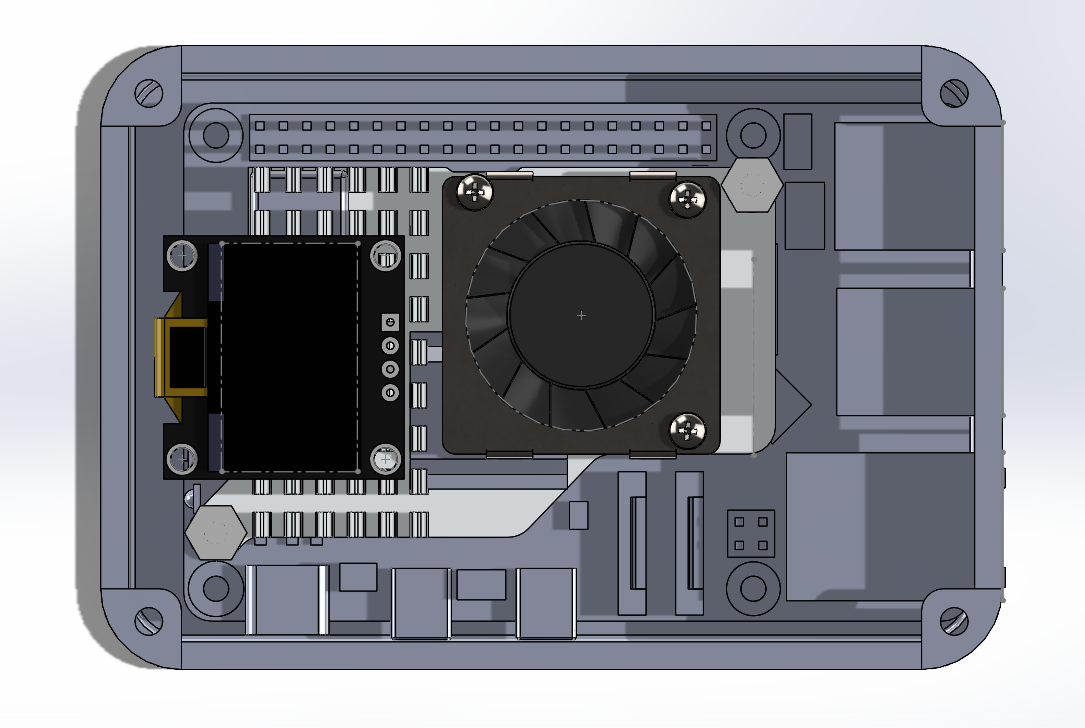
\includegraphics[width=\textwidth]{figures/cad/case_open.png}
        \caption{Vista de la carcasa sin tapa, mostrando el volumen interno y
        las zonas previstas para alojamiento de componentes.}
    \end{subfigure}
    \hfill
    \begin{subfigure}[t]{0.48\textwidth}
        \centering
        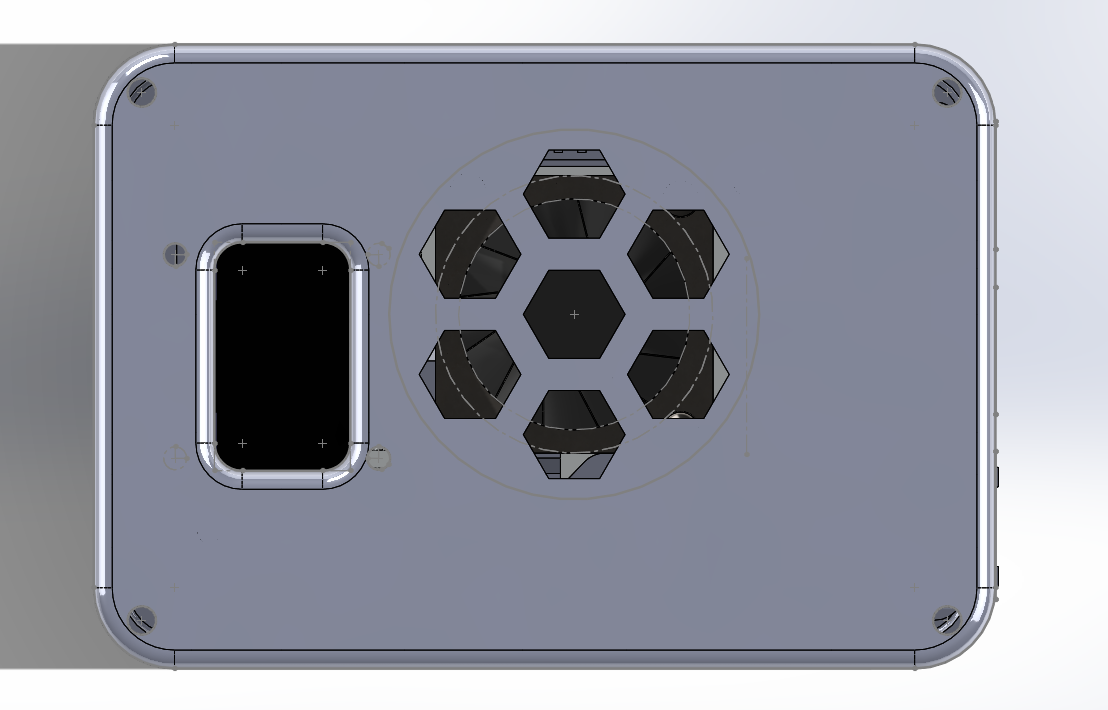
\includegraphics[width=\textwidth]{figures/cad/case_lid.png}
        \caption{Vista de la tapa de cierre diseñada para proteger el conjunto
        sin bloquear la ventilación ni los accesos principales.}
    \end{subfigure}
    \caption{Diseño 3D de la carcasa de protección desarrollado en SolidWorks
    2022. Se muestran (a) el cuerpo principal sin tapa y (b) la tapa del conjunto
    de protección. \textbf{Fuente:} Elaboración propia.}
    \label{fig:diseno_3d_proteccion_pi5}
\end{figure}

\section{Sistema de captura}

El sistema de captura integra el telescopio refractor, la cámara monocromática,
el elemento de atenuación solar y la interfaz de control ejecutada en la
Raspberry Pi 5. Su función es obtener imágenes fotosféricas en luz blanca,
almacenarlas localmente y dejarlas disponibles para preprocesamiento, inferencia
y sincronización posterior.

\subsection{Configuración de firmware}

La adquisición se implementa en Ubuntu~24 mediante el SDK de ZWO para cámaras
ASI sobre Raspberry Pi 5. Esta interfaz permite controlar por software la
exposición, ganancia, formato de imagen, región de interés y secuencias de
captura, evitando la operación manual durante la adquisición
\cite{zwoASILinuxManual,raspberryPi5Docs2026}.

La configuración de bajo nivel parte de verificar la arquitectura del sistema y
seleccionar la biblioteca compartida correspondiente del SDK. En una estación de
desarrollo x64 se utiliza la biblioteca de escritorio; en Raspberry Pi 5 se usa
la variante ARM compatible, típicamente la carpeta \texttt{armv8}. Esta distinción
es crítica porque la cámara se inicializa mediante \texttt{libASICamera2.so}; una
biblioteca compilada para otra arquitectura impediría abrir el dispositivo.

\begin{lstlisting}[language=bash,basicstyle=\footnotesize\ttfamily,breaklines=true,caption={Verificación de arquitectura y selección de biblioteca del SDK de ZWO.},label={lst:zwo-arquitectura}]
uname -m
ls SDK_ZWO/lib
# En Raspberry Pi 5 se selecciona la variante ARM compatible.
# Ejemplo: armv8.
\end{lstlisting}

Instalada la biblioteca, el entorno de ejecución se configura mediante
\texttt{ZWO\_ASI\_LIB}, variable que apunta a \texttt{libASICamera2.so} y permite
que los módulos basados en \texttt{zwoasi} localicen el controlador sin rutas
codificadas en el programa. Además, se actualiza la caché del sistema mediante
\texttt{ldconfig} para dejar la biblioteca disponible a los servicios de captura.

\begin{lstlisting}[language=bash,basicstyle=\footnotesize\ttfamily,breaklines=true,caption={Configuración de la biblioteca compartida del SDK de ZWO.},label={lst:zwo-biblioteca}]
export ZWO_ASI_LIB=ruta/del/sdk/armv8/libASICamera2.so
echo "ZWO_ASI_LIB=$ZWO_ASI_LIB"
ldconfig -v | grep ASICamera
\end{lstlisting}

También se incorpora una regla \texttt{udev} para el identificador USB del
fabricante ZWO, asociado al \texttt{idVendor} \texttt{03c3}. Esta regla asigna
permisos de acceso al dispositivo USB y evita que la captura dependa de ejecutar
el servicio con privilegios administrativos. En la práctica, el proceso de
arranque verifica la presencia de la cámara mediante detección USB, carga el SDK,
abre la comunicación con la ASI174MM Mini y solo entonces habilita las rutinas de
configuración de exposición, ganancia, formato de imagen y región de interés.

\begin{lstlisting}[language=bash,basicstyle=\footnotesize\ttfamily,breaklines=true,caption={Regla \texttt{udev} mínima para cámaras ZWO ASI.},label={lst:zwo-udev}]
SUBSYSTEM=="usb", ATTR{idVendor}=="03c3", \
  MODE="0666", GROUP="plugdev"
udevadm control --reload-rules
udevadm trigger
\end{lstlisting}

Sobre esta base se instalan las dependencias necesarias para captura y análisis
local: \texttt{zwoasi} para acceder al SDK, \texttt{opencv-python} para
operaciones de imagen, \texttt{numpy} para manejo matricial y \texttt{ultralytics}
cuando se requiere inferencia YOLO en el entorno de pruebas. Estas dependencias completan la configuración funcional del nodo al permitir detección de cámara, captura de imágenes y
generación de metadatos para la plataforma.

\begin{lstlisting}[language=bash,basicstyle=\footnotesize\ttfamily,breaklines=true,caption={Instalación de dependencias de adquisición y análisis local.},label={lst:zwo-dependencias}]
python -m pip install zwoasi opencv-python numpy ultralytics
python - <<'EOF'
import zwoasi as asi
print("SDK ZWO disponible")
EOF
\end{lstlisting}

\subsection{Captura de imagen}

El núcleo técnico del sistema es la transferencia eficiente de datos desde el
SDK nativo de ZWO hacia el flujo de procesamiento basado en \texttt{OpenCV}. Esta
capa organiza la lectura del sensor, la transferencia USB~2.0 y la conversión de
los datos crudos en matrices compatibles con visión artificial.

El proceso se ejecuta mediante un hilo especializado, de desarrollo propio,
\texttt{CameraWorker}, que opera como puente asíncrono entre la cámara y las
capas superiores del sistema. La adquisición invoca métodos de bajo nivel del SDK
para recuperar buffers crudos desde el bus USB~2.0. Estos buffers contienen la
información digitalizada por el sensor en formatos como RAW8 o RGB24,
inicialmente representada como flujos lineales de bytes.

La integración con \texttt{OpenCV} se realiza mediante \texttt{NumPy}. El buffer
se interpreta con \texttt{frombuffer} como una matriz unidimensional y luego se
reestructura mediante \textit{reshaping} según las dimensiones de la región de
interés (ROI). Así, el flujo binario se convierte en un \texttt{ndarray}
compatible con codificación, filtrado y análisis de imagen.

Para mantener una respuesta adecuada durante vista previa, enfoque y verificación
de exposición, las operaciones se ejecutan sobre datos residentes en memoria,
evitando escrituras intermedias en disco. Además, la adquisición concurrente
permite que \texttt{CameraWorker} mantenga el ciclo de captura mientras el backend
realiza compresión JPEG en tiempo real, generando datos optimizados para
transmisión y visualización local sin interrumpir la lectura del sensor.

\section{Conectividad y configuración de red local}
\label{sec:conectividad-hardware}

La robustez operativa en campo depende de una conectividad dual que no interfiera
con la adquisición. Para ello, la Raspberry Pi 5 opera como cliente de una red
externa y, simultáneamente, como punto de acceso inalámbrico para control local.
La interfaz \texttt{wlan0} se reserva para la conexión WiFi disponible, mientras
que la interfaz virtual \texttt{ap0} se dedica a la red privada del instrumento.

Esta separación permite acceso directo al prototipo aun sin Internet y mantiene
la posibilidad de sincronizar datos cuando la red externa esté disponible. La red
local se orienta al control inmediato, monitoreo y acceso al panel de operación;
la conexión externa se reserva para transferencia diferida, respaldo y consulta
remota de resultados.

La gestión del punto de acceso se realiza mediante \texttt{hostapd}. En esta
configuración se emplea el controlador \texttt{nl80211}, encargado de la
comunicación con el subsistema inalámbrico de Linux y el chip de radio de la
Raspberry Pi 5. El siguiente bloque resume los parámetros utilizados para
establecer la red privada del instrumento.

\begin{lstlisting}[language=bash,basicstyle=\footnotesize\ttfamily,breaklines=true,caption={Configuración del punto de acceso local mediante hostapd.},label={lst:hostapd-ap0}]
interface=ap0
driver=nl80211
ssid=Pi5_Observatory_Local
hw_mode=g
channel=11
wmm_enabled=1
macaddr_acl=0
auth_algs=1
ignore_broadcast_ssid=0
wpa=2
wpa_passphrase=Observatory2026
wpa_key_mgmt=WPA-PSK
wpa_pairwise=TKIP
rsn_pairwise=CCMP

# Stability optimizations
ieee80211n=1
# Optimized HT40 caps for channel compatibility
ht_capab=[SHORT-GI-20][DSSS_CCK-40]
\end{lstlisting}

Para automatizar la comunicación de los dispositivos conectados se emplea
\texttt{dnsmasq} como servicio local de DHCP y resolución de nombres. Este
componente asigna direcciones IP en la subred privada y resuelve el dominio local
asociado al panel de control, evitando que el operador deba recordar una dirección
IP específica.

La configuración se restringe a \texttt{ap0} para evitar interferencias con otras
interfaces de red. Además, define un rango DHCP acotado y establece la Raspberry
Pi 5 como puerta de enlace y servidor DNS. El dominio \texttt{observatory.local}
se resuelve hacia la dirección fija del nodo de control, facilitando el acceso al
backend y al panel local.

\begin{lstlisting}[language=bash,basicstyle=\footnotesize\ttfamily,breaklines=true,caption={Configuración de dnsmasq para asignación DHCP y resolución local.},label={lst:dnsmasq-ap0}]
# Only listen on the AP interface
interface=ap0
bind-dynamic

# DHCP Range (192.168.4.10 to 192.168.4.100)
dhcp-range=192.168.4.10,192.168.4.100,255.255.255.0,24h

# DHCP Options (3=Gateway, 6=DNS)
dhcp-option=3,192.168.4.1
dhcp-option=6,192.168.4.1

# Optimization for low latency
domain-needed
bogus-priv
no-resolv
local=/observatory.local/
address=/observatory.local/192.168.4.1
\end{lstlisting}

En conjunto, esta infraestructura permite que el nodo de observación funcione de
forma autónoma en campo. El operador accede mediante la red local y el dominio
\texttt{observatory.local} para controlar la captura y revisar servicios sin
conexión externa. Cuando existe Internet, la interfaz destinada a redes externas
habilita la sincronización diferida con la plataforma web sin comprometer el
enlace local de operación.